\chapter{Analysis chain}\label{ch:analysis}
%
For the PhotonStream data representation, as a new way of describing IACT data,
there is no reference analysis chain so far. The new possibilities of this
representation need new analysis structures and give way for new methods and
solutions. This work is therefore comparing different approaches to solve the
tasks of this analysis. A schematic representation of the analysis flow is
shown in \autoref{fig:analysis}.
%
\begin{figure}[H]
  \centering
  \begin{tikzpicture}[node distance = 1.5cm, auto]
    \node (f1) [feature, xshift=-2.0cm] {PhotonStream};
    \node (f2) [LP, xshift=2.0cm] {Largest Pulse};
    \draw[line width=0.7mm, below of=f1] (-4.2,0.7) -- (4.2,0.7);
    \node (s1) [astep, xshift=-4.0cm, anchor=west, below of=f1] {calibration};
    \node (f3) [feature, below of=f1] {\begin{varwidth}{9em}\centering{Extracting single photons}\end{varwidth}};
    \node (f4) [LP, below of=f2] {\begin{varwidth}{9em}\centering{Identifying large pulses}\end{varwidth}};

    \node (f5) [feature, below of=f3] {DBSCAN};
    \node (f6) [LP, below of=f4] {\begin{varwidth}{9em}\centering{pixel-based thresholds}\end{varwidth}};
    \node (s2) [astep, below of=s1] {image cleaning};
    \node (f7) [feature, below of=f5] {parameter set A};
    \node (f8) [LP, below of=f6] {parameter set B};
    \node (s3) [astep, below of=s2] {parametrization};
    \node (f9) [both, below of=f7, xshift=2.0cm] {AICT Tools~\cite{aicttools}};
    \node (s4) [astep, below of=s3] {separation};
    \node (f10) [both, below of=f9] {AICT Tools~\cite{aicttools}};
    \node (s5) [astep, below of=s4] {energy \& origin reconstruction};

    \draw [arrg] (f3) -- node[anchor=east] {} (f5);
    \draw [arrg] (f3) -- node[anchor=east] {} (f6);
    \draw [arry] (f4) -- node[anchor=east] {} (f6);
    \draw [arrg] (f5) -- node[anchor=east] {} (f7);
    \draw [arrg] (f6) -- node[anchor=east] {} (f7);
    \draw [arry] (f6) -- node[anchor=east] {} (f8);
    \draw [arrg] (f7) -- node[anchor=east] {} (f9);
    \draw [arry] (f8) -- node[anchor=east] {} (f9);
    \draw [arry, color=cyan] (f9) -- node[anchor=east] {} (f10);
  \end{tikzpicture}
  \caption{Schematic flow of the different analysis steps of this analysis. The PhotonStream analysis uses different calibrations (\autoref{sec:phs}) and a different cleaning (DBSCAN) than the LP representation. Nonetheless, the PhotonStream data contains all information neccessary to apply the LP pixel-based threshold cleaning on the calibrated data.}
  \label{fig:analysis}
\end{figure}
%
To generate PhotonStream data a different calibration is needed. As described
in \autoref{sec:phs}, instead of finding large pulses and calculating the data
coordinates, the time series data is turned into single photons. The additional
information of the PhotonStream is then used to clean the image in the
threedimensional spacetime via the DBSCAN algorithm, rather than by setting
timing and PE thresholds for air-shower pixels. Nonetheless, the PhotonStream
data contains all that is neccessary to perform this pixel-based cleaning
instead. Therefore, this analysis is investigating said cleaning on
PhotonStream data as well as the DBSCAN cleaning. The parametrization of the
events in PhotonStream representation uses a subset of the features of the LP
analysis, to have the best comparability. Especially the additional timing
information of the PhotonStream is not used in feature generation for this
analysis. The different analysis steps shown in \autoref{fig:analysis} are
described in the following section. The results of the combinations of these
steps as represented by the arrows in \autoref{fig:analysis} are then evaluated
in \autoref{ch:results}.

\section{Image Cleaning on the PhotonStream}\label{sec:phs_clean}
%
As pointed out in \autoref{ch:iact} the Cherenkov-light of air-showers shows a
very specific topology. The emitted photons are coherent in space and time:
they originate from a single very high energetic and therefore very fast
primary particle and thus appear in a very brief time window of a few
nanoseconds. Furthermore, the characteristic Cherenkov-angle under which the
light is emitted, creates a light cone, which, when projected to the
$x$-$y$-plane of the camera causes the specific elliptical shape. Both of these
topological features are mandated by the physical process and can therefore be
unrestrictedly used for the cleaning. Background events like ambient light or
starlight do not show these characteristics and tend to appear randomly.

The threedimensional $xyt$-representation of the PhotonStream, called point-cloud, quantifies photons with exactly those three observables. Thus, a cleaning
within the threedimensional space-time can heavily use the known topology.
Within the point-cloud, an air-shower will appear as a very dense cluster of
photons, surrounded by a merely isotropic distribution of background photons.
These characteristics of shower events in the PhotonStream representation
naturally suggest a density-based clustering algorithm as the cleaning method
of choice. The two challenges at hand are the choice of a suited algorithm and
a well defined metric to make the threedimensional spacetime usable.

\subsection{Air-showers in the Point-Cloud}
%
The threedimensional spacetime of the PhotonStream and its representation as a
point-cloud eventually mixes spatial dimensions with time. While this is
physically motivated, defining distances in such a space is not trivial. They
are highly dependent on the chosen metric, which defines how time corresponds to
space. This already implies that the choice of metric contains certain
assumptions and can be adapted to specific preferences. The essential parameter
is the factor $\alpha$, which transfers time to space and vice versa:
%
\begin{equation}
  c_{t} = \alpha \cdot t \, .
  \label{eq:metric}
\end{equation}
%
The choice of this parameter e.g. gives the possibility to prefer spatial
distance over timing information, or the opposite. The spacetime of the
point-cloud is quantized in all its three dimensions: the pixels of the camera
define the spatial grid, whereas the time slices, each event is binned to, do so
for the timing information. When trying to separate air-showers from
background via the density of the shower's photons, the distance plays the
essential role. The natural way to equalize between space and time is to adapt
to the photon distribution of a typical air-shower along each axis. So, by
choosing
%
\begin{equation}
  \alpha = 0.35\cdot10^9\,\si{\degree\per\second}\, ,
\end{equation}
%
the one-dimensional density distribution of photons along the coordinates
$c_x$, $c_y$ and $c_t$ is the same. With this metric, the distance between two
photons $a$ and $b$ is defined as
%
\begin{equation}
  d_{a,b} = \sqrt{(c_x^a - c_x^b)^2 + (c_y^a - c_y^b)^2 + (c_t^a - c_t^b)^2}
\end{equation}

The twodimensional projections of the point-cloud within this metric are shown
in \autoref{fig:pc} for an example air-shower event. With the calculated
degree-equivalent of time the air-shower shows a similar distribution in
each dimension.
%
\begin{figure}[H]
  \centering
  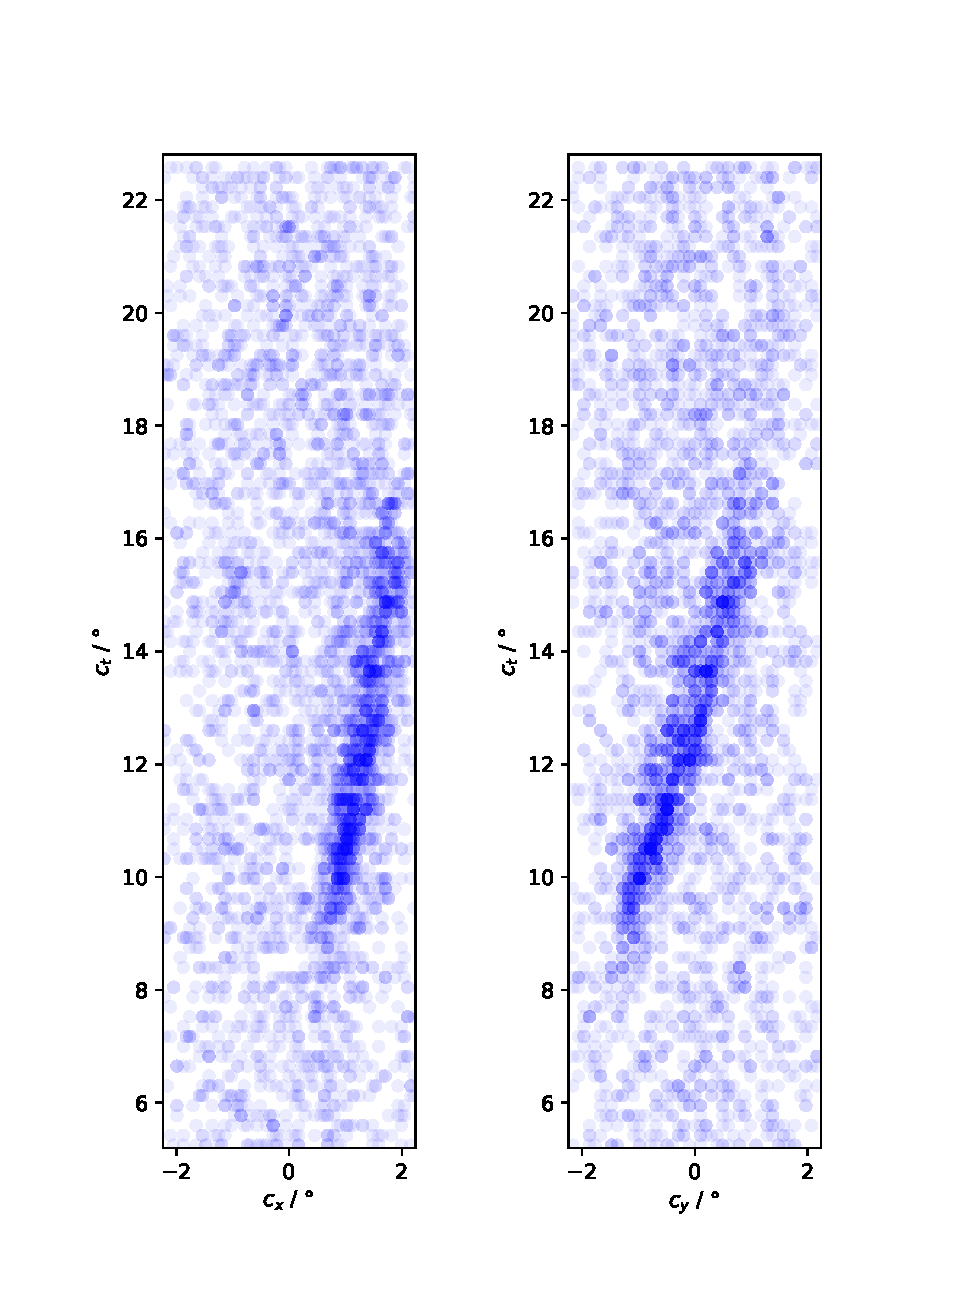
\includegraphics[width=0.6\textwidth, angle=-90]{Plots/point_cloud.pdf}
  \caption{Twodimensional projections of the point-cloud using the metric described above.}
  \label{fig:pc}
\end{figure}
%

\subsection{Density-based Clustering with DBSCAN}
%
To find clusters of photons within the space described above, the PhotonStream
uses the \textit{density-based algorithm for discovering clusters with noise}
(DBSCAN) \cite{DBSCAN}. The DBSCAN is well suited for finding air-showers with the
PhotonStream's observables, when choosing the right parameter set for the algorithm. This
algorithm either assigns each extracted photon to one of potentially multiple
clusters or identifies it as a night-sky-background photon. There are no
assumptions on the shape, location or number of the clusters. The algorithm is
characterized by only two parameters.
%
\begin{description}[]
  \item[m] the minimum number of photons to make up a cluster
  \item[$\symbf{\varepsilon}$] the maximum distance between two photons to be considered dense
\end{description}
%
These two parameters represent the specific topology of the air-shower events
by giving limits on typical shower sizes and spreads in spacetime. For
air-shower events recorded by FACT the best choice was found to be $m = 20$ and
$\varepsilon = \SI{0.45}{\degree}$. So, to survive the cleaning, every found
cluster must at least contain 20 photons within a maximum distance of
$\SI{0.45}{\degree}$ to the respective closest photon. The algorithm determines
the clusters by iterating over the photons in 4 steps:
%
\begin{enumerate}
  \item loop over photons until a dense region with at least $m$ photons is found
  \item add photons to the newly found cluster that are within distance $\varepsilon$ or connected via a chain of dense photons
  \item if nothing to add to cluster restart 1. with leftover photons
  \item mark all photons not assigned to any dense cluster as night-sky-background
\end{enumerate}
%
This way every photon is either belonging to a cluster of an air-shower, or
discarded as background. This determination is taking place in the whole space
of observables the whole time. There are no intermediate steps, only taking
single observables into account, which very much represents a way to find
air-showers in a space well suited for describing them. Furthermore, this way
single photons are selected rather than specific pixels. When expecting
background photons also within signal pixels, this should yield a cleaned image,
closer to the true air-shower image. An example event before and after cleaning
is shown in \autoref{fig:event_u} and \autoref{fig:event_c}.
%
% \begin{figure}
%   \begin{subfigure}{\textwidth}
%     \centering
%     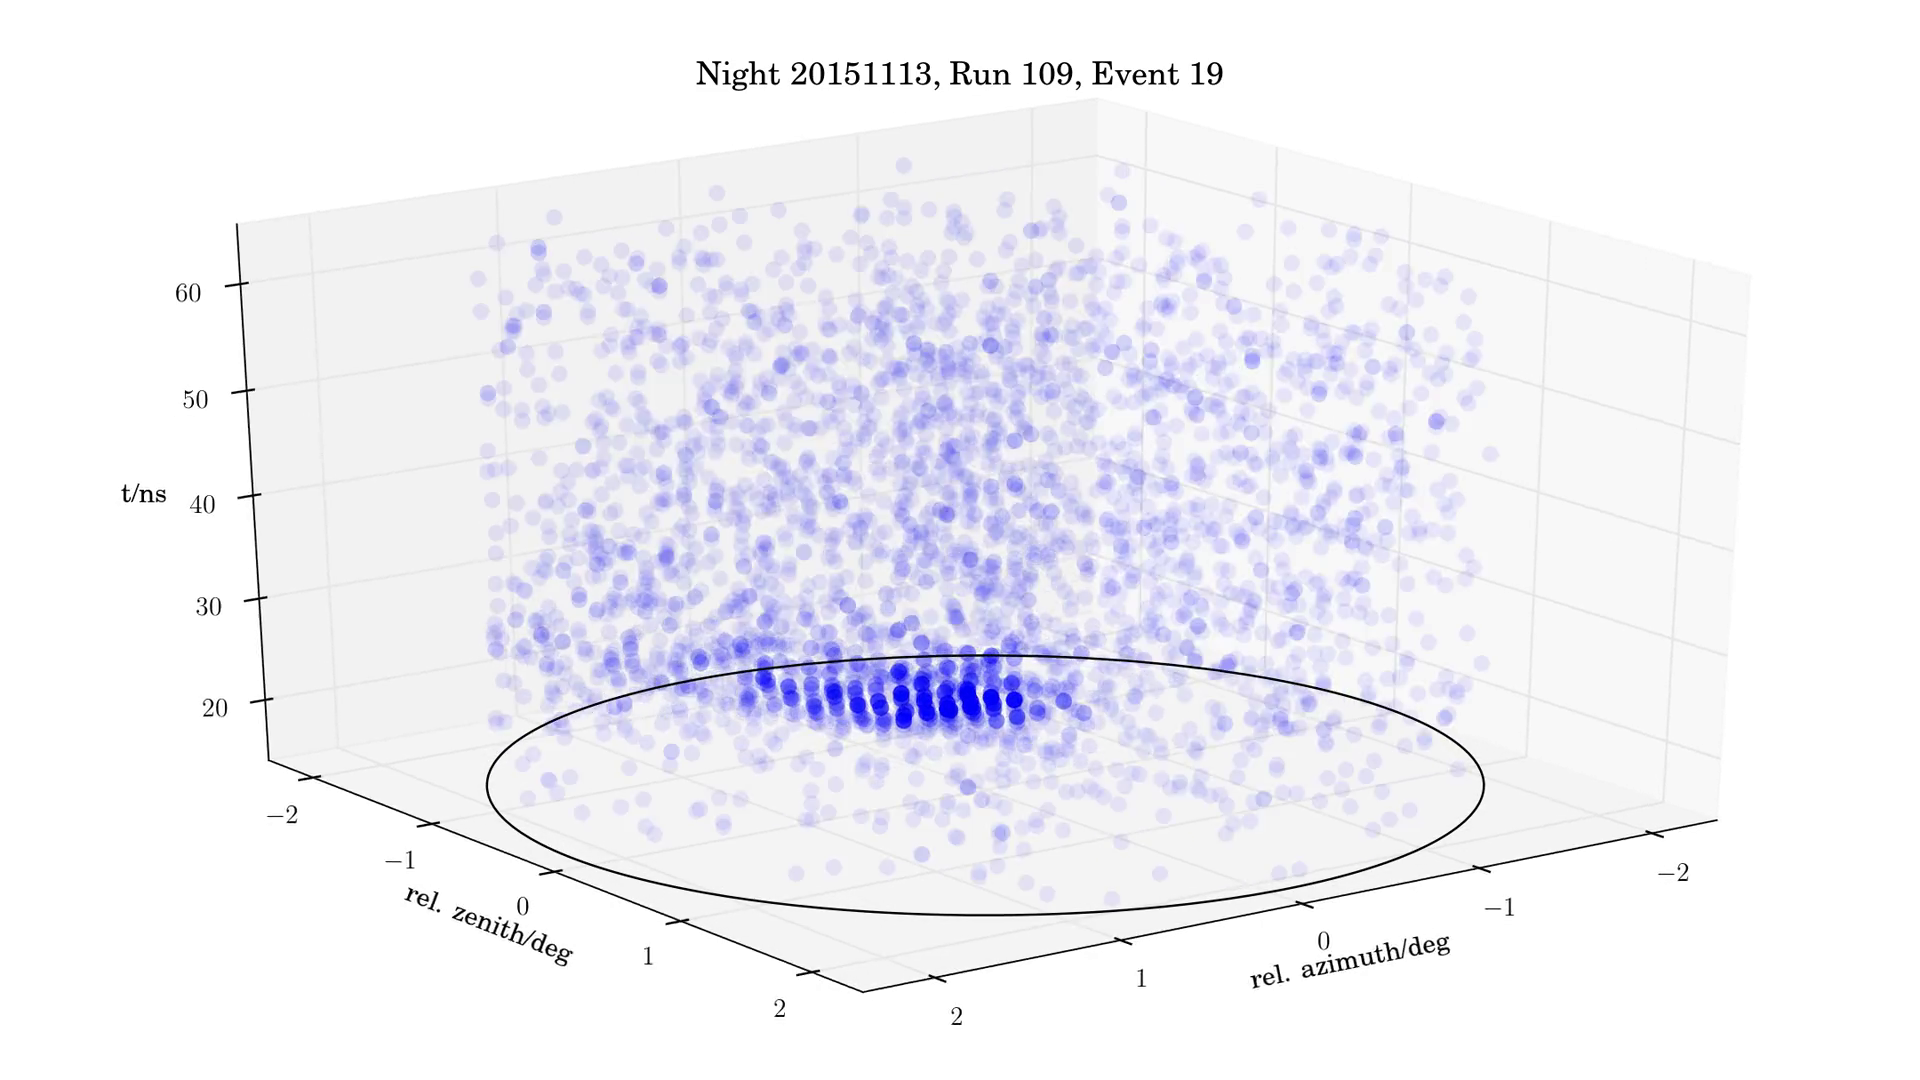
\includegraphics[width=0.9\textwidth]{Plots/event2.png}
%   \end{subfigure}
%   \begin{subfigure}{\textwidth}
%     \centering
%     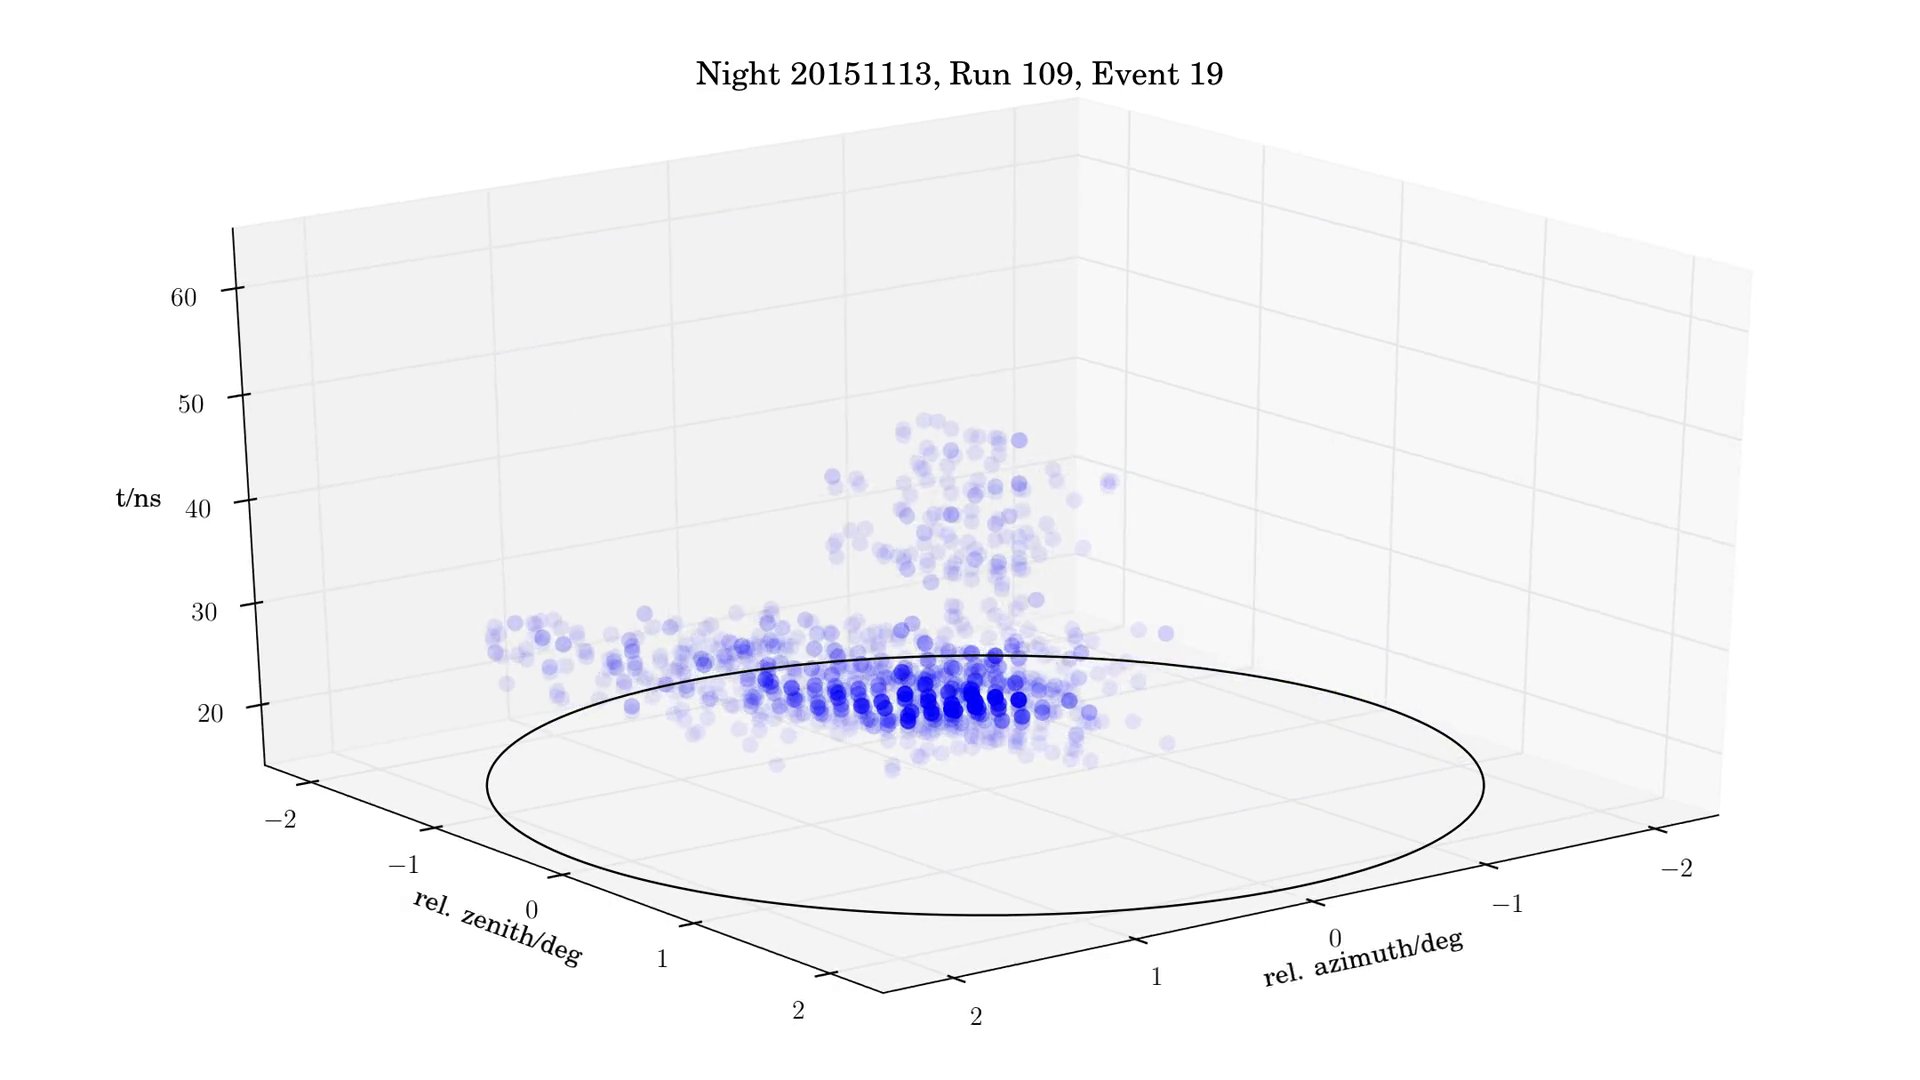
\includegraphics[width=0.9\textwidth]{Plots/event1.png}
%   \end{subfigure}
%   \caption{Event represented by the 3-dimensional point cloud of the Photonstream. Every blue sphere represents a measured photon in the corresponding time slice and pixel. The right figure shows the remaining photons after cleaning.}
%   \label{fig:event}
% \end{figure}
%
%
\begin{figure}
  \centering
  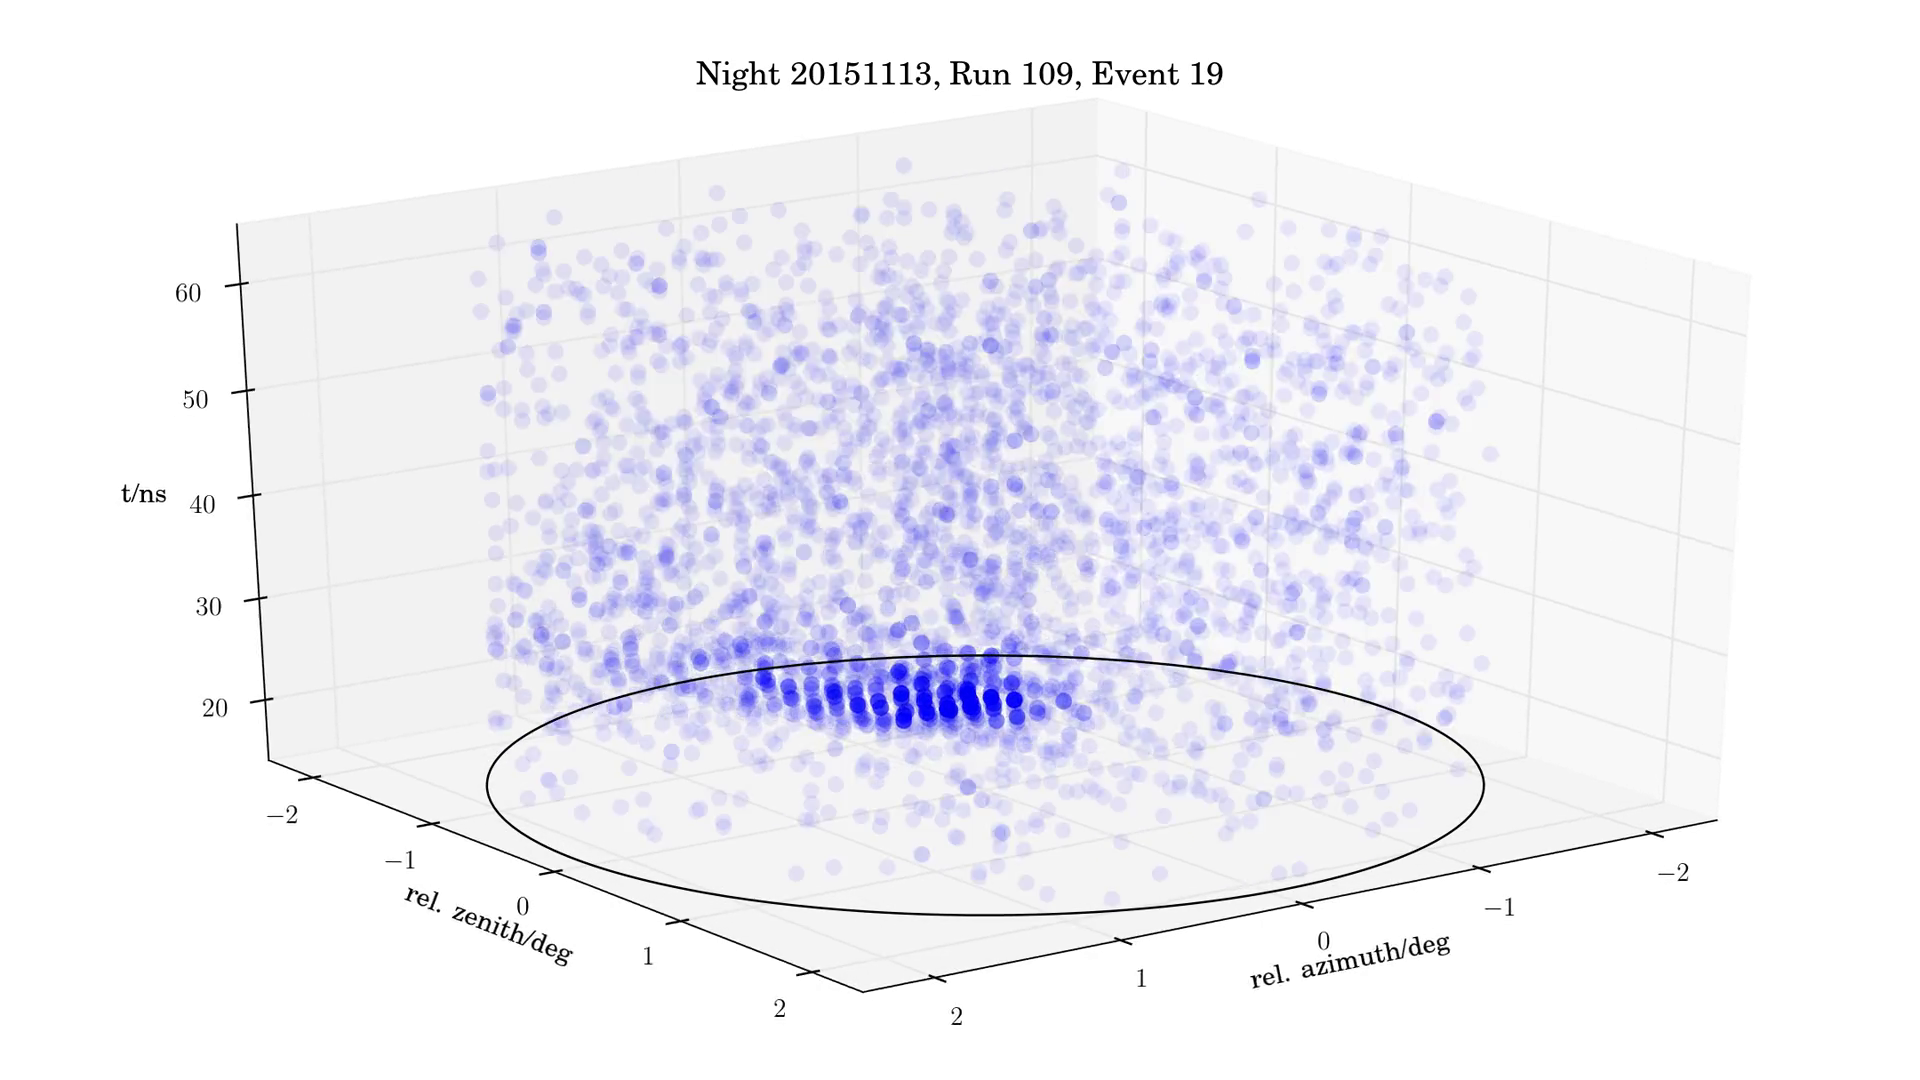
\includegraphics[width=0.9\textwidth]{Plots/event2.png}
  \caption{Uncleaned event represented by the 3-dimensional point cloud of the Photonstream. Every blue sphere represents a measured photon in the corresponding time slice and pixel.}
  \label{fig:event_u}
\end{figure}
\begin{figure}
  \centering
  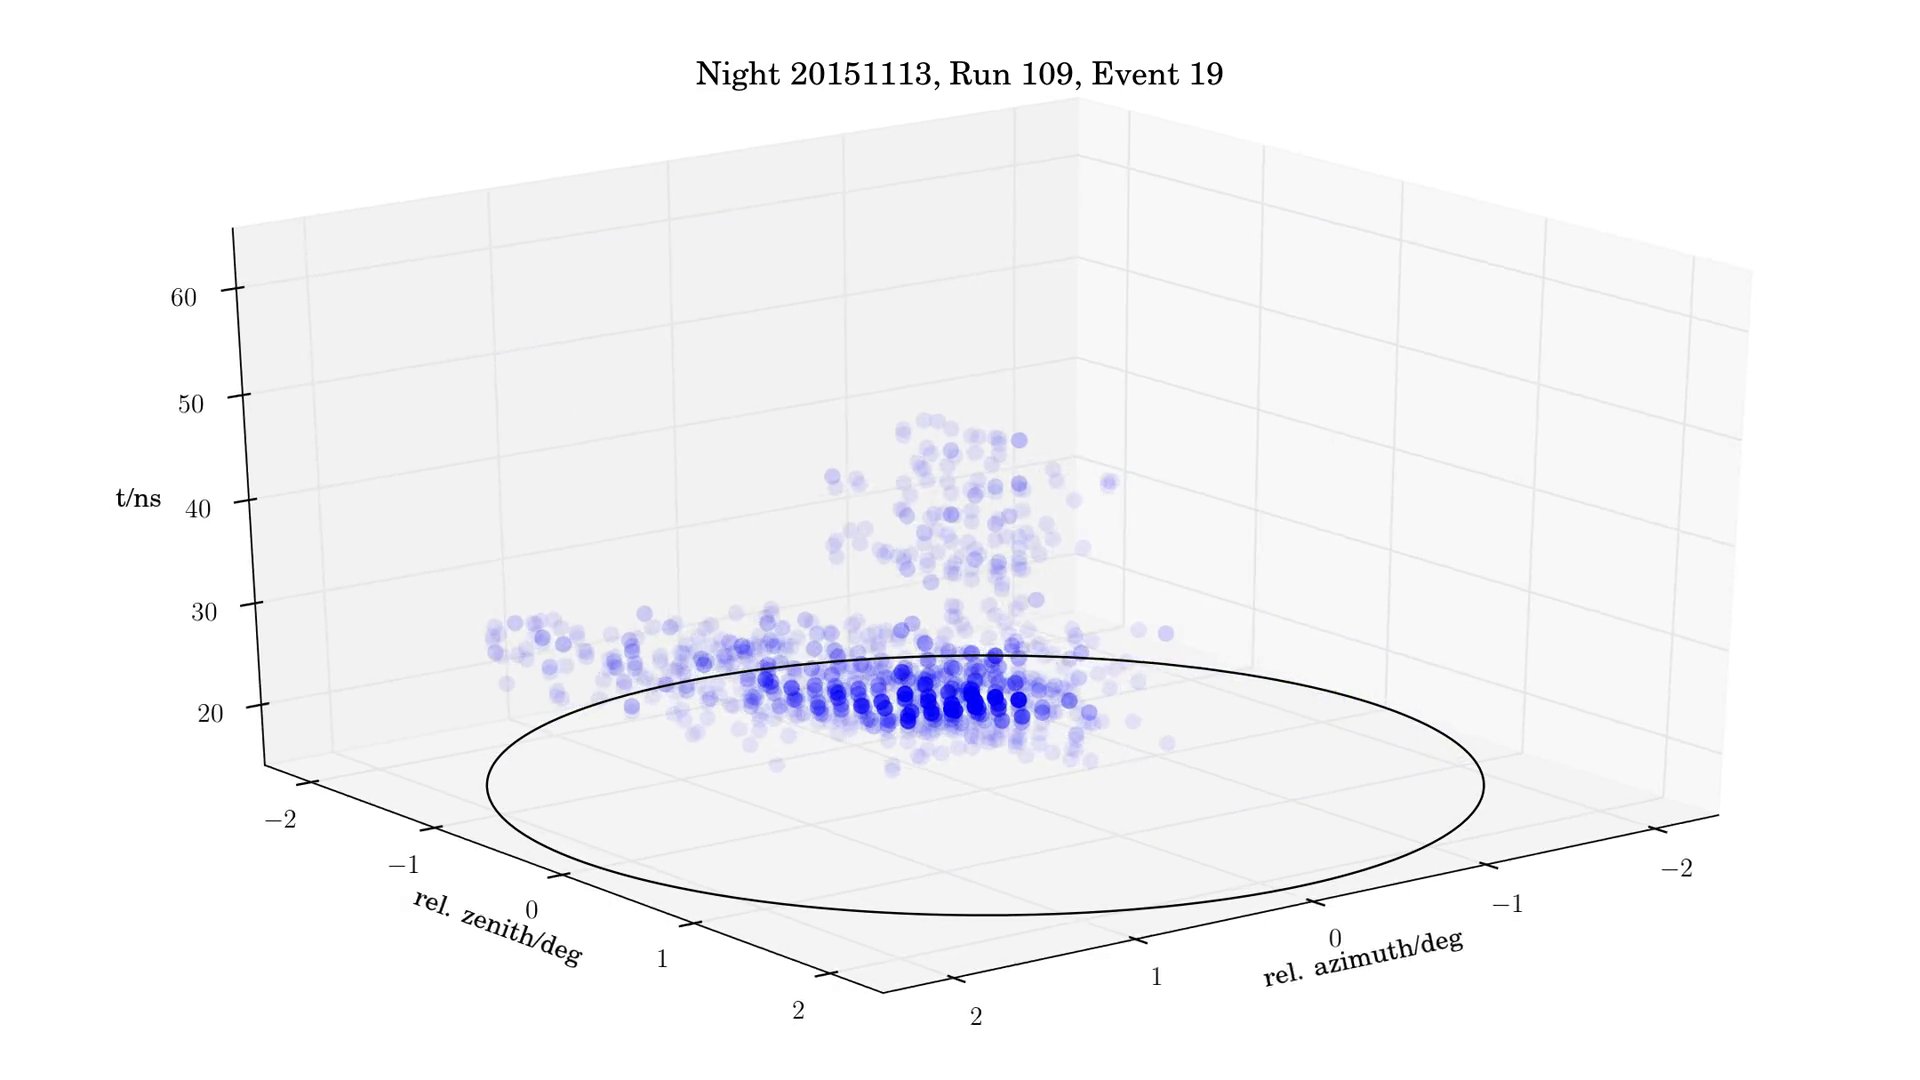
\includegraphics[width=0.9\textwidth]{Plots/event1.png}
  \caption{Cleaned event represented by the 3-dimensional point cloud of the Photonstream. Every blue sphere represents a measured photon in the corresponding time slice and pixel.}
  \label{fig:event_c}
\end{figure}
%

\section{Parametrization of Events}
\label{sec:params}
%
For the classical analysis the detected images need to be parametrized. The
learning algorithms work with specific features rather than the whole image,
although there are indeed ways to analyze whole images.

The parametrization that is most frequently chosen for IACT data is based on
the one proposed by Hillas~\cite{Hillas}. It operates on the two dimensional
images recorded by the cameras, calculating features of the air-shower pixels.
In the original publication these features were used to successfully analyze
images on a 37-pixels camera. The parametrization is based on the light
distribution among the air-shower pixels by calculating the eigenvalue
decomposition of the covariance. A graphical representation of a typical
air-shower image is shown in \autoref{fig:hillas}.
%
\begin{figure}
  \centering%
  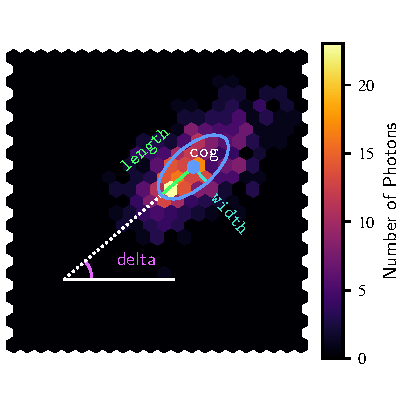
\includegraphics[width=0.6\textwidth]{Plots/hillas.pdf}%
  \caption{A graphical representation of a typical air-shower image \cite{maxhillas}. The figure shows the number of photons per pixel of an air-shower. The dotted
  line represents the air-shower axis. It corresponds to the line minimising the
  sum of perpendicular angular distance, weighted by the number of photons per
  pixel. The standard deviations along this axis and the perpendicular axis are
  the two features called \texttt{length} and \texttt{width}. The center of
  gravity (\texttt{cog}) of the air-shower image is the two dimensional weighted
  mean of all shower pixels.}%
  \label{fig:hillas}%
\end{figure}
%
The figure shows the number of photons per pixel of an air-shower. The dotted
line represents the air-shower axis. It corresponds to the line minimising the
sum of perpendicular angular distance, weighted by the number of photons per
pixel. The standard deviations along this axis and the perpendicular axis are
the two features called \texttt{length} and \texttt{width}. The center of
gravity (\texttt{cog}) of the air-shower image is the two dimensional weighted
mean of all shower pixels. The position and orientation of the shower is also
characterized by the angle \texttt{delta}. It is the angle between the shower
axis and the camera's $x$-axis. The \texttt{size} of the air-shower simply
corresponds to the sum of photons measured in all air-shower pixels.

To further parametrize the air-showers also higher order statistical moments of
the light distributions are used. Those are the third (\texttt{skewness}) and
fourth (\texttt{kurtosis}) statistical moments of the air-shower photons along
the two axes defined above. The values are calculated in a rotated system in
respective to the camera system, so that the two main axes define the
coordinate axes.
%
\begin{align}
  \text{skew}(X) &= \text{E}\left[\left(\frac{X-\mu}{\sigma}\right)^3\right] \label{eq:skew} \\
  \text{kurt}(X) &= \text{E}\left[\left(\frac{X-\mu}{\sigma}\right)^4\right]  \label{eq:kurt}
\end{align}
%
Additional to the \texttt{size} of an air-shower the number of pixels
\texttt{n\_pixel} containing air-shower photons is used as a feature. Since
there might be more than one cluster in an air-shower event, especially for
hadron showers, the ratio of the cluster sizes (\texttt{cluster\_size\_ratio})
is used for the gamma hadron separation.
%
\section{Reconstruction of the Source Position}
\label{sec:source_pos}%
%
FACT is a single telescope and therefore has no stereoscopic features to
determine the origin of the cosmic ray showers. Thus, specific techniques only
using the features of the air-shower images have to be performed. In this
analysis the so called disp-method is used. It estimates the origin position of
the cosmic gamma-rays by estimating the \texttt{disp} and the \texttt{sign}. The two
dimensional problem of determining $x$ and $y$ coordinates is turned into a
regression task and a classification task. The estimated source position within
the camera's image is assumed to be on the shower's main axis. To find this
position the first step is to estimate the distance to the \texttt{cog} of the
air-shower. \texttt{disp} is representing that distance of the estimated source inside
the camera. As described earlier the fraction of \texttt{width} and \texttt{length} is dependant
on the angle under that the air-shower is hitting the camera. Thus, it is
\enquote{pointing} to the cosmic origin of the shower.

The second step is to determine the direction of \texttt{disp} along
the main axis. As shown in \autoref{fig:disp_amb} the distance \texttt{disp} alone is
not sufficient to determine the source position, but an additional direction is
needed. Otherwise there remains an ambiguity, as shown in the two examples.
The assumption of the origin position being on the shower axis reduces this
task to a binary classification of the sign of \texttt{disp}.
%
\begin{figure}
  \begin{subfigure}{0.5\textwidth}
    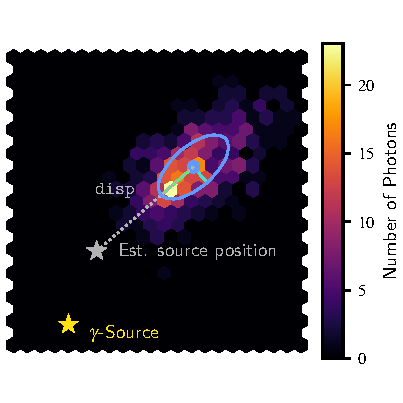
\includegraphics[width=\textwidth]{Plots/hillas_4.pdf}
  \end{subfigure}
  \begin{subfigure}{0.5\textwidth}
    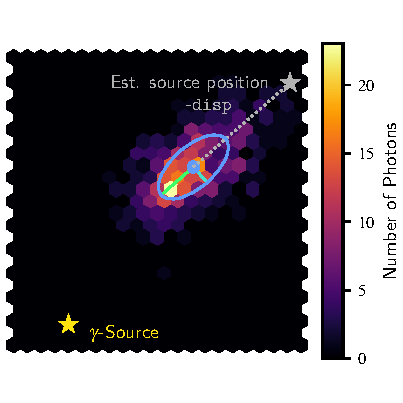
\includegraphics[width=\textwidth]{Plots/hillas_5.pdf}
  \end{subfigure}
  \caption{Ambiguity of the reconstruction direction along an example shower's main axis \cite{maxhillas}. The calculated \texttt{disp} can be applied to two directions along the shower axis and therefore needs to be determined as well.}
  \label{fig:disp_amb}
\end{figure}
%
The reconstructed source position can then be validated by comparing it to the
known source position as shown in \autoref{fig:disp}. The calculated distance
between the both is labelled $\theta$ and source specific.
%
\begin{figure}
  \centering%
  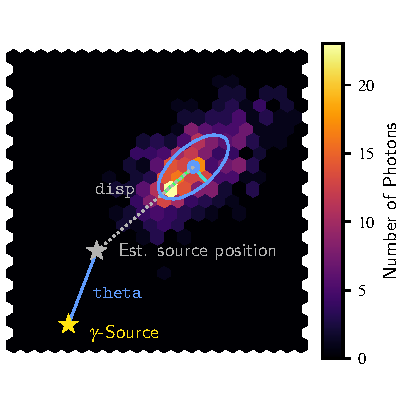
\includegraphics[width=0.6\textwidth]{Plots/hillas_disp.pdf}%
  \caption{Result of the reconstruction of the source position using the disp-method \cite{maxhillas}. From the reconstructed source position the distance $\theta$ to the true source position can be calculated to validate the reconstruction.}%
  \label{fig:disp}%
\end{figure}
%
\section{Image Cleaning with Pixel-Based Thresholds}
\label{sec:thresh}
%
When using the largest pulse representation (LP), a different cleaning is
used. Since the PhotonStream is a different representation, of course the
optimal cleaning differs. When cleaning LP data an algorithm working on the PE
of the pixels is used. This cleaning is based on the assumption that air-shower
images contain a certain minimum number of photons per pixel and appear in a
quite small range of time and space within one event. It does not contain any
assumptions on the number of clusters per event, but with the mentioned
assumptions generally implies a certain topology within the camera's
coordinates. Since arrival times in this representation are properties per
pixel the time correlation has to be given between neighboring pixels. The
algorithm executes the following steps \cite{facttools}:
%
\begin{enumerate}
  \item find pixels containing more photons than an upper threshold $t_1$ (5~p.e.)
  \item remove pixels with less than 2 neighbors above $t_1$
  \item add neighbors of remaining pixels that are above a lower threshold $t_2$ (2.5~p.e.)
  \item remove pixels that have less than 2 neighbors arriving in $\SI{5}{\nano\second}$ time window
  \item remove single pixels with less than 2 neighbors
  \item remove pixels that have less than 2 neighbors inside a $\SI{5}{\nano\second}$ time window
\end{enumerate}
%
The remaining pixels are considered to be the cleaned image. When projecting
the PhotonStream data into a camera image and calculating the mean arrival
times per pixel, unlike the threedimensional DBSCAN, this cleaning can
equivalently be performed on PhotonStream data.


\section{Energy Estimation and Signal-Background Separation}
%
The generated features (\autoref{sec:params}) are used for the estimation of
the primary particle's energy and the classification of the particle via
machine learning algorithms as described in \autoref{ch:ML}. To generate and
train the random forests the framework \texttt{aict-tools} \cite{aicttools} is
used. It provides executables for the configuration, training and application
of machine learning tasks on IACT data. The executables use the popular python
machine learning library \texttt{scikit-learn}~\cite{scikit-learn}, which comes
with a plethora of supervised and unsupervised machine learning algorithms,
data preparation tools and evaluation functions. All three major tasks of this
analysis can be performed by these tools on the used data set.
